\chapter{Evaluation}
\label{chap:evaluation}

For demodularization to be useful, it should improve performance of modular programs.
To test whether or not this is the case, we created benchmarks to test the speed of demodularized programs versus their modular counterparts.
We also compare the results with the cross-module inliner included in Racket.
We show improvements in the size of programs through the use of a dead-code elimination algorithm.
Finally, we discuss further improvements that demodularization can enable.

\section{Racket Optimizer}

The Racket optimizer included a cross-module inliner in version 5.2. 
This inliner accomplishes many of the same improvements that the demodularizer does.
The inliner does have limitations on the size of functions that it will inline, so with large functions demodularization is still preferable.
We compare the results with the inliner turned off, with the inliner turned on, and with demodularization.
The demodularized programs are also run through the existing Racket optimizer.

\section{Testing Setup}

The tests were run on a MacBook Pro (2GHz Intel i7 processor, 8GB Memory) in OS X Yosemite, using Racket v6.2. 
Each test was run 5 times and an average of the results was taken.

\section{Micro-benchmarks}

The micro-benchmarks for demodularization involve a module that calls a function from another module, which calls a function from another module, and so on for the number of modules in the test. 
The function call happens in a loop to get times that are significant.
The full test generation code can be found in Appendix~\ref{chap:benchmarks}.
Figure~\ref{fig:micro-results} shows the results of running these benchmarks with different numbers of modules.
\begin{figure}
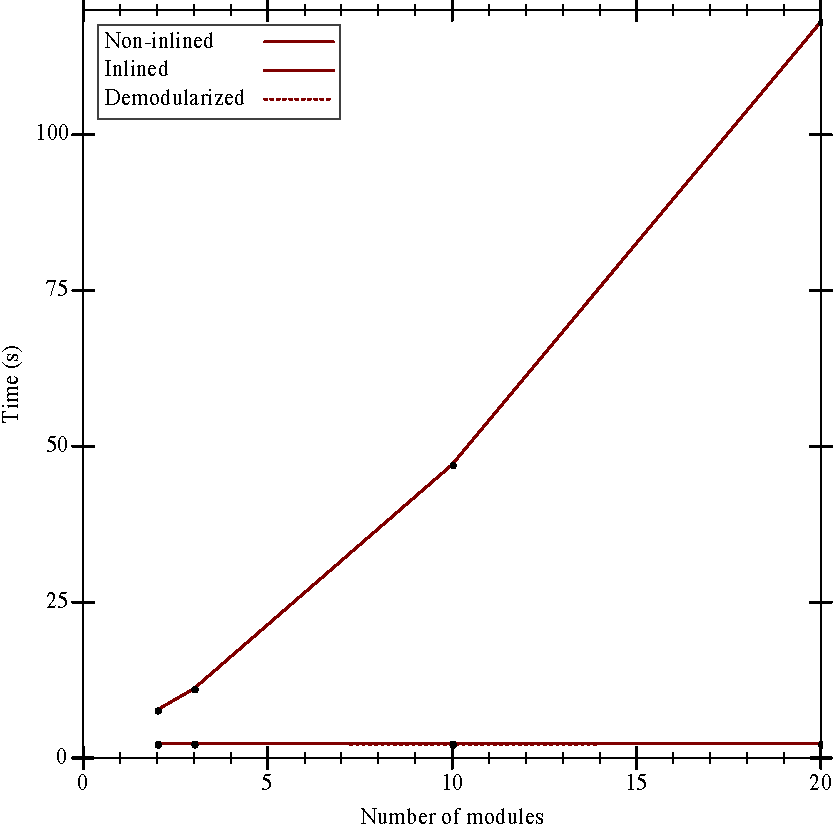
\includegraphics{figures/micro-results}
\caption{Results from micro-benchmarks}
\label{fig:micro-results}
\end{figure}
Without inlining, the micro-benchmarks increase in a linear fashion with an increase in the number of modules.
With inlining, the micro-benchmarks stay at a constant speed.
It would be possible to trick the inliner by creating large function bodies of unused code, but that is not the goal of the micro-benchmarks.
With demodularization, the micro-benchmarks also stay at a constant speed, with a slightly better speed than inlining.

\section{Real World Benchmarks}
For real world benchmarks we selected programs that would terminate deterministically and that used multiple modules.
One of the programs we tested was a program that uses the Racket xml library to read large xml files.
The program can be found in Appendix~\ref{chap:benchmarks}.
For test data, we used astronomical data from NASA~\cite{nasa}. 
The second program we tested is a benchmark for the Redex tool.
Redex is a library that allows users to build and test semantic models.
The benchmark is also included in Appendix~\ref{chap:benchmarks}.
Figure~\ref{fig:macro-results} shows the results of running demodularization on larger programs.
\begin{figure}
\caption{Results from real world benchmarks}
\label{fig:macro-results}
\end{figure}

\section{Dead Code Elimination}
As an experiment, we implemented an unsound dead code elimination algorithm for demodularized programs.
It identifies all uses of toplevel definitions in the body of the demodularized program and eliminates all other toplevels.
The reason it is unsound is because although some toplevels may not be referenced directly in the program, they may be needed for side-effects that they have.
These side-effects may include setting up global objects or tables that will be referenced by the program, or I/O operations.
In order to make the dead code elimination algorithm sound, we would need to identify primitives that can have side-effects and include any toplevels that use those primitives.
Figure~\ref{fig:dead-code} shows how much smaller programs become after running the dead code elimination algorithm on them.
\begin{figure}
\caption{Dead code elimination results}
\label{fig:dead-code}
\end{figure}

\section{Further Optimizations}

Having access to the whole-program at once enables optmizations that currently are not implemented by the Racket optimizer.
For example, any optimizations that rely on Control-Flow Analysis (CFA) require access to the whole program.
Demodularization enables these sorts of optmiziations to be performed on modular programs.

